% \chapter{Klasteryzacja i topografia wag}
% \label{chap:klasteryzacja}

% \section{Zastosowanie algorytmów gęstościowych (HDBSCAN) do separacji domen semantycznych}

% \section{Badanie zależności i sąsiedztwa faktów w architekturze modelu}

% \section{Mapowanie relacji korelacyjnych między neuronami warstw liniowych a wyekstrahowanymi klastrami SAE}

\chapter{Klasteryzacja cech i mapowanie domen semantycznych na neurony MLP}
\label{chap:klasteryzacja}
Ekstrakcja cech opisana w poprzednim rozdziale tworzy słownik kierunków w przestrzeni reprezentacji analizowanego modelu językowego wraz z przykładami ich aktywacji. Aby wykorzystać ten słownik do budowy modeli dziedzinowych, konieczne jest jednak wykonanie dwóch dodatkowych kroków: segregacja cech w semantycznie spójne grupy -- dalej określane jako domeny oraz ustalenie związku budujących domeny cech z neuronami modelu bazowego. W niniejszym rozdziale przedstawiony zostanie ów proces triażu domen semantycznych, ich ocena i wybór kandydatów do dalszych eksperymentów, a następnie ich mapowanie na neurony pośrednie części MLP. Analiza dotyczy modelu \textit{Gemma 3 270M} i autoenkodera dla warstwy $9$, opisanego w podrozdziale~\ref{sec:adaptacja_gemma_scope}. Jej wynikiem są zbiory cech domenowych oraz rankingi neuronów, stanowiące podstawę późniejszego pruningu i tworzenia ekspertów. 

\section{Reprezentacja cech i klasteryzacja domen metodą HDBSCAN}
\label{sec:triage_klasteryzacja}
Punktem wyjścia jest zapis analizy cech SAE, obejmujący ich identyfikatory, statystyki, tokeny promowane (\textit{logit lens}) oraz konteksty użycia cech. W ukończonej analizie Gemmy przetworzono $99\,999\,989$ tokenów ze zbioru \textit{The Pile} \cite{gao_2020_pile_800gb_dataset_diverse} i zaobserwowano aktywność $16\,343$ spośród $16\,384$ cech. Brak zaobserwowanej aktywacji nie musi oznaczać tutaj, że dana cecha jest martwa -- czyli  pozostaje nieaktywna dla wszystkich możliwych wejść. Istnieje duża szansa, że dana aktywacja nie wystąpiła po prostu w analizowanym korpusie tekstu. Z racji jednak na małą ilość takich nieaktywnych cech zostały one pominięte w dalszej analizie. \newline
Pierwszy badany sposób triażu, opisywał cechę poprzez tokeny promowane przez jej kierunek dekodera. Kierunek ten jest rzutowany na macierz wyjściową modelu, a następnie zachowywane są najwyżej ocenione tokeny. Po odrzuceniu tokenów specjalnych i zastosowaniu filtrów leksykalnych powstaje rzadka macierz cecha--token. Wagi są korygowane odwrotną częstością występowania tokenu w opisach cech, a wiersze normalizowane normą $L_2$. Reprezentacja ta jest jednak niedokładna: bezpośrednie rzutowanie kierunku z warstwy pośredniej pomija dalsze bloki transformera i końcową normalizację. W przeprowadzonych próbach klastry były często zdominowane przez fragmenty słów, język lub format tekstu, co utrudniało wyodrębnienie domen tematycznych. \newline
Z tego powodu właściwy już sposób triażu, wykorzystany w dalszych etapach oparto na kontekstach aktywacji. Dla każdej zaobserwowanej cechy połączono zapisane konteksty jej najsilniejszych aktywacji w jeden dokument. Dokumenty przekształcono w wektory TF-IDF (ang. \textit{term frequency--inverse document frequency}) \cite{salton_1988_term_weighting_approaches_automatic_text_retrieval}, w których częstość słowa jest ważona jego rzadkością w całym zbiorze dokumentów cech. Zastosowano logarytmiczne skalowanie częstości, normalizację $L_2$, sprowadzenie liter do małych oraz usunięcie angielskich słów funkcyjnych. Słownik ograniczono do $50\,000$ terminów występujących w co najmniej trzech dokumentach i nie więcej niż $20\%$ dokumentów. Niepustą reprezentację uzyskano dla $16\,342$ cech. Do opisu każdej cechy zachowano $64$ terminy o najwyższych wagach; sama klasteryzacja korzystała z pełnej macierzy TF-IDF, bez tego ograniczenia. \newline
Przed klasteryzacją macierz poddano redukcji wymiarowości stosując obcięty rozkład według wartości osobliwych (ang. \textit{Truncated Singular Value Decomposition}, SVD). Pozwoliło to zmniejszyć wymiar reprezentacji przy zachowaniu rzadkiego formatu danych wejściowych. W przebiegu bazowym zastosowano $50$ składowych, a uzyskane wektory ponownie znormalizowano. Grupowanie wykonano algorytmem HDBSCAN \cite{campello_2013_hdbscan,mcinnes_2017_hdbscan}, opisanym w podrozdziale~\ref{sec:redukcja_wymiarowosci}, z metryką euklidesową. Przyjęto minimalny rozmiar klastra równy $40$, parametr \texttt{min\_samples} równy $10$ oraz wybór klastrów metodą \texttt{leaf}, wyodrębniającą końcowe grupy z hierarchii. Liczba domen nie była narzucana na etapie klasteryzacji. \newline
W konfiguracji bazowej uzyskano $23$ klastry, a około $79{,}1\%$ niepustych wektorów oznaczono jako szum. Cech tych nie przypisywano później do najbliższej domeny. Tak duży udział szumu ogranicza pokrycie słownika SAE, ale pozwala uniknąć wymuszania grup dla cech, które przy zadanych parametrach nie tworzą dostatecznie gęstych skupisk. Dalsze dostrajanie autoenkodera lub procesu analizy, a także wybór modelu z większą ilością parametrów mógłby pozwolić zmniejszyć udział szumu w ogólnej liczbie cech. Jednakże na potrzeby badań niniejszej pracy uzyskane pokrycie zostało uznane za wystarczające.

\section{Ocena stabilności i wybór domen do dalszych eksperymentów}
\label{sec:wybor_domen}
Dla każdego klastra wyznaczany jest centroid w pierwotnej przestrzeni reprezentacji oraz spójność, czyli średnie podobieństwo cosinusowe cech do tego centroidu. Jeżeli $C$ oznacza zbiór identyfikatorów cech klastra, a $v_i$ jest znormalizowanym wektorem cechy, to:
\[
c_C=\frac{\sum_{i\in C}v_i}{\left\|\sum_{i\in C}v_i\right\|_2},
\qquad
q_C=\frac{1}{|C|}\sum_{i\in C}v_i^{\mathsf T}c_C.
\]
Pomocniczy wynik $q_C\log(1+|C|)$ łączy spójność z licznością grupy. \newline
Dla analizy cech modelu \texttt{Gemma 3} wykonano sześć wariantów triażu, dostrajając parametry: liczbę składowych SVD na $30$ lub $80$, ziarno losowe na $1$ lub $2$, a także minimalny rozmiar klastra na $20$ lub $80$; w ostatnim wariancie zwiększono również \texttt{min\_samples} do $20$. Dla każdego klastra bazowego znajdowano najbardziej zbliżony zbiór cech w danym przebiegu, mierząc nakładanie indeksem Jaccarda \cite{jaccard_1901_etude_distribution_florale}:
\[
J(C,C')=\frac{|C\cap C'|}{|C\cup C'|}.
\]
Średnia najlepsza wartość Jaccarda z sześciu porównań służyła do ważenia wyniku bazowego. Pozwalało to odróżnić grupy powtarzalne od skupisk silnie zależnych od konfiguracji. Dodatkowo zapisywano skorygowany indeks Randa (ang. \textit{Adjusted Rand Index}, ARI) \cite{hubert_1985_comparing_partitions}, zarówno dla wszystkich niepustych cech, jak i dla cech przypisanych do klastrów w obu porównywanych przebiegach. \newline
Ranking stanowił podstawę ręcznego przeglądu reprezentatywnych terminów i kontekstów, po którym wybrano i zatwierdzono sześć domen zestawionych w tabeli~\ref{tab:wybrane_domeny}. Cztery z nich odpowiadają tematyce tekstów, natomiast matematyka i Python obejmują także łatwo rozpoznawalne własności notacji lub składni. Z tego powodu pełnią dodatkowo rolę kontroli, w której separacja może być prostsza niż dla domen opartych wyłącznie na znaczeniu. Nazwy nadano po interpretacji klastrów; ich numery są identyfikatorami nadanymi podczas przebiegu triażu. W aneksie~\ref{appendix:katalog_cech_gemma} przedstawiono po jednej przykładowej cesze wyodrębnionej przez SAE dla modelu \textit{Gemma 3 270M} z każdej z sześciu wybranych domen, wraz z interpretacją, tokenami aktywującymi i promowanymi oraz przykładami kontekstów aktywacji. 
\begin{table}[htbp]
\centering
\small
\begin{tabular}{lrrr}
\toprule
Domena & Klaster & Liczba cech & Średni Jaccard \\
\midrule
Prawo i orzecznictwo & 20 & 161 & $0{,}889$ \\
Biomedycyna & 17 & 396 & $0{,}837$ \\
Sport & 16 & 117 & $0{,}759$ \\
Polityka i wiadomości & 22 & 123 & $0{,}696$ \\
Matematyka / zapis LaTeX & 15 & 322 & $0{,}893$ \\
Python & 5 & 149 & $0{,}718$ \\
\bottomrule
\end{tabular}
\caption{Domeny wybrane do mapowania na neurony MLP. Stabilność oznacza średnie najlepsze nakładanie klastra bazowego z klastrami w sześciu alternatywnych konfiguracjach.}
\label{tab:wybrane_domeny}
\end{table}
% TODO: zanalizować konieczność poniższego fragmentu:
Przykłady wydobyte z analizy SAE lub dobrane na podstawie słownictwa klastra pozostają materiałem diagnostycznym: korzystają z tej samej informacji, która posłużyła do utworzenia domen. Do dalszych etapów przygotowano zatem osobne korpusy dziedzinowe z zapisanym pochodzeniem danych i oddzielonym zbiorem końcowym (ang. \textit{holdout}). Dobór neuronów wykorzystuje część rozwojową; zbiór końcowy służy późniejszej ocenie gotowego rozwiązania. Rozdzielenie zbiorów ogranicza bezpośredni przeciek danych.

\section{Mapowanie aktywacji domenowych na neurony MLP}
\label{sec:mapowanie_domen_mlp}

% TODO: sprawdzić bramkowanie Gemma 
% Cecha SAE, współrzędna strumienia rezydualnego i neuron pośredni MLP należą do trzech różnych przestrzeni. W analizowanej Gemmie ich wymiary wynoszą odpowiednio $16\,384$, $640$ i $2048$.  Mapowanie realizowane jest przez przechwycenie wejścia projekcji wyjściowej MLP. Model \texttt{Gemma} używa bramkowanego MLP, gdzie jest to wejście modułu \texttt{down\_proj}:
Cecha SAE, współrzędna strumienia rezydualnego i neuron pośredni MLP należą do trzech różnych przestrzeni. W analizowanej Gemmie ich wymiary wynoszą odpowiednio $16\,384$, $640$ i $2048$. Celem mapowania jest ustalenie związku między aktywacją neuronów MLP a łącznym pobudzeniem cech SAE należących do wybranej domeny. \newline
Przechwytywane są więc aktywacje na wejściu projekcji wyjściowej \texttt{down\_proj}. Gemma wykorzystuje bramkowane MLP (ang. \textit{gated MLP}), w którym dwie projekcje przetwarzają ten sam wektor wejściowy: jedna, po zastosowaniu funkcji aktywacji, reguluje elementowo wartości drugiej. Ich iloczyn tworzy wektor aktywacji neuronów pośrednich, następnie rzutowany z powrotem do wymiaru strumienia rezydualnego:
\[
a(t)=\operatorname{act}(W_{\mathrm{gate}}u(t))
\odot W_{\mathrm{up}}u(t),
\]
gdzie $u(t)$ oznacza wejście MLP dla pozycji tokenu $t$, a $\odot$ -- iloczyn elementowy. Każda współrzędna $a_j(t)$ odpowiada tej samej osi wewnętrznej w obu projekcjach wejściowych i projekcji wyjściowej. Równocześnie przechwytywany jest strumień rezydualny po tym samym bloku, kodowany następnie przez SAE. \newline
Niech $z_i(t)$ oznacza aktywację cechy SAE, a $C_d$ -- zbiór cech domeny $d$. W wykorzystanym wariancie sygnał domenowy ma postać:
\[
s_d(t)=\sum_{i\in C_d}z_i(t).
\]
Suma zachowuje łączny poziom pobudzenia klastra, ale jej wartość zależy od liczby i skali cech, dlatego nie powinna być bezpośrednio porównywana między domenami jako miara ich ważności. \newline
Mapowanie przeprowadzono na wspólnym, losowo przemieszanym korpusie tekstów wszystkich sześciu domen. Dla każdego tokenu obliczono aktywacje MLP i sygnały wszystkich domen, uzyskując macierz $A\in\mathbb{R}^{T\times H}$ oraz macierz $S\in\mathbb{R}^{T\times K}$, gdzie $T$ oznacza liczbę tokenów, $H$ -- szerokość MLP, a $K$ -- liczbę domen. W wykonanym przebiegu wykorzystano $60\,000$ tokenów z $351$ tekstów, przy $H=2048$ i $K=6$. Wspólny zbiór obserwacji umożliwia porównywanie związków neuronu z różnymi domenami i pozwala współdzielić obliczenia modelu. \newline
Przebieg mapowania przedstawiono na rysunku~\ref{fig:mapowanie_domen_mlp}. Dwa punkty pomiaru dotyczą tego samego przejścia modelu, a wiersze obu macierzy odpowiadają tym samym pozycjom tokenów.
\begin{figure}[htbp]
\centering
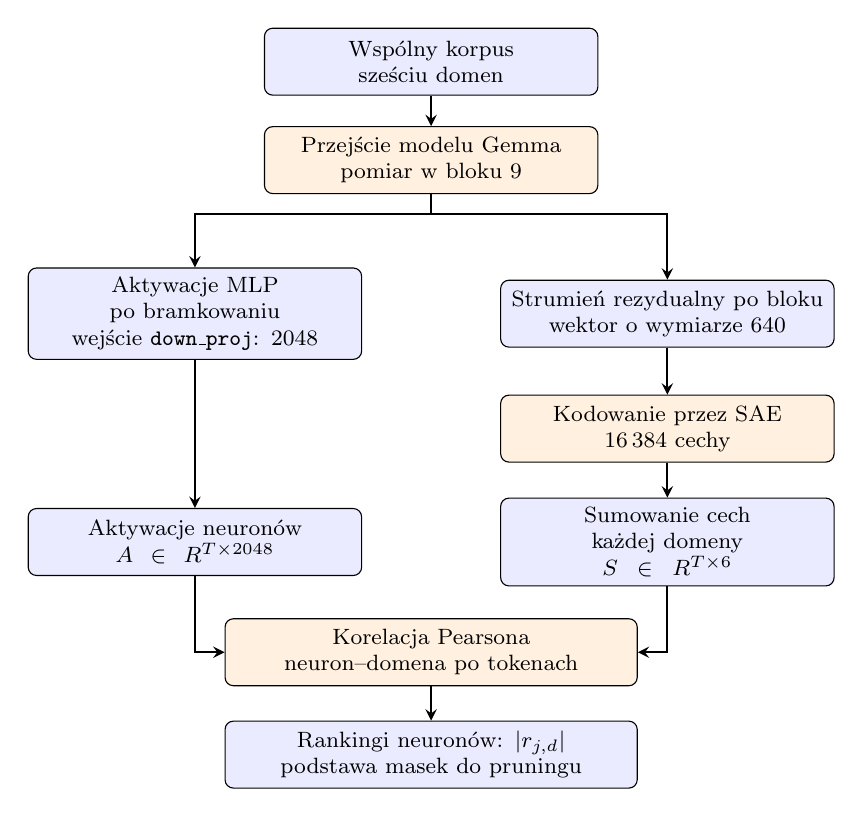
\begin{tikzpicture}[
    box/.style={draw, rounded corners=3pt, text width=4.0cm,
                minimum height=0.85cm, align=center, font=\footnotesize\linespread{1}\selectfont},
    data/.style={box, fill=blue!8},
    proc/.style={box, fill=orange!12},
    arr/.style={->, >=stealth, thick}
]
\node[data] (texts) at (0,0) {Wspólny korpus sześciu domen};
\node[proc] (model) at (0,-1.25) {Przejście modelu Gemma\\pomiar w bloku $9$};
\node[data] (mlp) at (-3,-3.2) {Aktywacje MLP po bramkowaniu\\wejście \texttt{down\_proj}: $2048$};
\node[data] (resid) at (3,-3.2) {Strumień rezydualny po bloku\\wektor o wymiarze $640$};
\node[proc] (sae) at (3,-4.66) {Kodowanie przez SAE\\$16\,384$ cechy};
\node[data] (matrix) at (-3,-6.1) {Aktywacje neuronów\\$A\in\mathbb{R}^{T\times2048}$};
\node[data] (signals) at (3,-6.1) {Sumowanie cech każdej domeny\\$S\in\mathbb{R}^{T\times6}$};
\node[proc, text width=5cm] (corr) at (0,-7.5) {Korelacja Pearsona\\neuron--domena po tokenach};
\node[data, text width=5cm] (rank) at (0,-8.8) {Rankingi neuronów: $|r_{j,d}|$\\podstawa masek do pruningu};
\draw[arr] (texts) -- (model);
\draw[arr] (model.south) -- ++(0,-0.25) -| (mlp.north);
\draw[arr] (model.south) -- ++(0,-0.25) -| (resid.north);
\draw[arr] (mlp) -- (matrix);
\draw[arr] (resid) -- (sae);
\draw[arr] (sae) -- (signals);
\draw[arr] (matrix.south) |- (corr.west);
\draw[arr] (signals.south) |- (corr.east);
\draw[arr] (corr) -- (rank);
\end{tikzpicture}
\caption{Schemat mapowania domen SAE na neurony MLP. $T$ oznacza liczbę analizowanych tokenów po usunięciu paddingu. Lewa gałąź dostarcza aktywacji neuronów, a prawa sygnałów domenowych wyznaczonych ze strumienia rezydualnego po bloku. Strzałki przedstawiają przepływ danych analitycznych.}
\label{fig:mapowanie_domen_mlp}
\end{figure}
Dla każdej pary neuron--domena obliczono współczynnik korelacji Pearsona:
\[
r_{j,d}=\frac{\sum_t(a_j(t)-\bar{a}_j)(s_d(t)-\bar{s}_d)}
{\sqrt{\sum_t(a_j(t)-\bar{a}_j)^2}\sqrt{\sum_t(s_d(t)-\bar{s}_d)^2}}.
\]
Statystyki są akumulowane blokami w podwójnej precyzji, bez tworzenia dodatkowej, wycentrowanej kopii pełnej macierzy aktywacji. Brak wariancji daje wynik niezdefiniowany, a niemal całkowity brak pobudzenia domeny jest sygnalizowany przed dalszym wykorzystaniem mapowania. Rankingi do pruningu oparto na $|r_{j,d}|$, uwzględniając zarówno dodatnie, jak i ujemne zależności. \newline
Na tych samych danych sprawdzono również selektywność sygnałów SAE: po uśrednieniu aktywacji w obrębie tekstu porównano daną domenę ze wszystkimi pozostałymi. Uzyskane wartości ROC-AUC mieściły się w przedziale od $0{,}957$ do $1{,}000$, a wszystkie domeny spełniły przyjęte kryterium AUC co najmniej $0{,}60$. \newline
Wyniki mapowania zapisano jako wspólną macierz aktywacji, sygnały SAE, identyfikatory tekstów i pozycji tokenów oraz tabele korelacji dla wszystkich $2048$ neuronów. Zestaw ten pozwala w kolejnym etapie wyznaczyć domenowe maski zachowania neuronów i zastosować je spójnie do odpowiednich projekcji MLP. Nie wymusza się rozłączności masek: ten sam neuron może być związany z kilkoma domenami.